% Options for packages loaded elsewhere
\PassOptionsToPackage{unicode}{hyperref}
\PassOptionsToPackage{hyphens}{url}
\documentclass[
  11pt,
  a4paper,
]{article}
\usepackage{xcolor}
\usepackage[margin=22mm]{geometry}
\usepackage{amsmath,amssymb}
\setcounter{secnumdepth}{-\maxdimen} % remove section numbering
\usepackage{iftex}
\ifPDFTeX
  \usepackage[T1]{fontenc}
  \usepackage[utf8]{inputenc}
  \usepackage{textcomp} % provide euro and other symbols
\else % if luatex or xetex
  \usepackage{unicode-math} % this also loads fontspec
  \defaultfontfeatures{Scale=MatchLowercase}
  \defaultfontfeatures[\rmfamily]{Ligatures=TeX,Scale=1}
\fi
\usepackage{lmodern}
\ifPDFTeX\else
  % xetex/luatex font selection
\fi
% Use upquote if available, for straight quotes in verbatim environments
\IfFileExists{upquote.sty}{\usepackage{upquote}}{}
\IfFileExists{microtype.sty}{% use microtype if available
  \usepackage[]{microtype}
  \UseMicrotypeSet[protrusion]{basicmath} % disable protrusion for tt fonts
}{}
\makeatletter
\@ifundefined{KOMAClassName}{% if non-KOMA class
  \IfFileExists{parskip.sty}{%
    \usepackage{parskip}
  }{% else
    \setlength{\parindent}{0pt}
    \setlength{\parskip}{6pt plus 2pt minus 1pt}}
}{% if KOMA class
  \KOMAoptions{parskip=half}}
\makeatother
\usepackage{graphicx}
\makeatletter
\newsavebox\pandoc@box
\newcommand*\pandocbounded[1]{% scales image to fit in text height/width
  \sbox\pandoc@box{#1}%
  \Gscale@div\@tempa{\textheight}{\dimexpr\ht\pandoc@box+\dp\pandoc@box\relax}%
  \Gscale@div\@tempb{\linewidth}{\wd\pandoc@box}%
  \ifdim\@tempb\p@<\@tempa\p@\let\@tempa\@tempb\fi% select the smaller of both
  \ifdim\@tempa\p@<\p@\scalebox{\@tempa}{\usebox\pandoc@box}%
  \else\usebox{\pandoc@box}%
  \fi%
}
% Set default figure placement to htbp
\def\fps@figure{htbp}
\makeatother
\setlength{\emergencystretch}{3em} % prevent overfull lines
\providecommand{\tightlist}{%
  \setlength{\itemsep}{0pt}\setlength{\parskip}{0pt}}
\usepackage{bookmark}
\IfFileExists{xurl.sty}{\usepackage{xurl}}{} % add URL line breaks if available
\urlstyle{same}
\hypersetup{
  pdftitle={Baker\textquotesingle s theorem I: building an auxiliary function},
  pdfauthor={GPT-6.1 Sol (OpenAI), Ultra},
  hidelinks,
  pdfcreator={LaTeX via pandoc}}

\title{Baker\textquotesingle s theorem I: building an auxiliary
function}
\author{GPT-6.1 Sol (OpenAI), Ultra}
\date{October 2026}

\providecommand{\Eta}{\mathrm{H}}
\begin{document}
\maketitle

\emph{Draft. Public domain (CC0).}

The proof will compare two measurements of the same value: complex
analysis makes it small, while arithmetic gives a lower limit if it is
nonzero. For that comparison to work, the values under consideration
must be algebraic after a controlled normalization. Ordinary derivatives
of exponential functions introduce logarithms, so choosing the right
derivatives is the first construction problem.

We begin with a hypothetical relation between two logarithms and examine
its diagonal jets. That calculation explains the separate variables in
Baker's auxiliary function. We then pass to any number of logarithms,
count the equations over a number field, and choose the polynomial
degree so that both the dimension count and the coefficient size have
room. The resulting function and its estimates are the inputs to
\href{../TR-BAKER-03.html}{\emph{Baker's theorem II: extrapolation and
the end of the proof}}.

We use the integer-matrix form of Siegel's lemma proved in
\href{../../TR-TRANS/TR-TRANS-05.html}{\emph{Siegel's lemma, analytic
estimates and the six exponentials theorem}}, Lemma 5.1 and equation
(5.2). The integral-basis theorem is proved in
\href{../../NT-ANT/discriminants-and-integral-bases.html}{\emph{Discriminants
and integral bases}}, Theorem 2.3; the norm's integrality and product of
conjugates are proved in
\href{../../NT-ANT/algebraic-integers-and-rings-of-integers.html}{\emph{Algebraic
integers and rings of integers}}, Section 3. Elementary complex
differentiation supplies the analytic identities. The several-variable
construction and the qualitative independence theorem are Baker's. The
freely accessible {[}Waldschmidt 2003{]} lectures explain the normalized
derivations and repeated extrapolation, including the algebraic constant
term and arbitrary complex logarithms. {[}Waldschmidt 2000{]} supplies
the height and box-principle arguments; {[}Sutherland 2021{]} supplies
proofs of the lattice and norm facts used above. The explanations of
normalized jets, integral coordinates and the parameter window below
make the roles of the choices explicit.

\subsection{1. The statement and the hypothetical
relation}\label{the-statement-and-the-hypothetical-relation}

\textbf{Theorem 2.1 (Baker).} Let \(\alpha_1,\ldots,\alpha_n\) be
nonzero algebraic numbers, and choose arbitrary logarithms \(\ell_j\)
with \(e^{\ell_j}=\alpha_j\). If \(\ell_1,\ldots,\ell_n\) are linearly
independent over \(\mathbb Q\), then

\[
1,\ell_1,\ldots,\ell_n
\]

are linearly independent over \(\overline{\mathbb Q}\).

Theorem 2.1 is the theorem to be proved across this lesson and the next.
It is not an input to the construction below. Suppose it fails. A
relation has the form

\[
\beta_0+\beta_1\ell_1+\cdots+\beta_n\ell_n=0,
\qquad \beta_j\in\overline{\mathbb Q},
\]

with coefficients not all zero. Some coefficient of a logarithm is
nonzero: otherwise \(\beta_0=0\) too. Relabel and divide to arrange
\(\beta_n=-1\). Thus

\[
\ell_n=\beta_0+\sum_{r=1}^{n-1}\beta_r\ell_r. \tag{2.1}
\]

All \(\ell_j\) are nonzero because they are rationally independent. Fix
the number field

\[
K=\mathbb Q(\alpha_1,\ldots,\alpha_n,\beta_0,\ldots,\beta_{n-1}),
\qquad D=[K:\mathbb Q].
\]

Constants in this lesson may depend on these fixed numbers and on the
chosen logarithms. They do not depend on the large integer \(h\)
introduced later.

The important feature of (2.1) is exponential, not just linear. For
integers \(\lambda_j\), define

\[
\gamma_r=\lambda_r+\lambda_n\beta_r\quad(1\le r<n).
\]

Then

\[
e^{\lambda_n\beta_0 z}\prod_{r<n}e^{\gamma_r\ell_r z}
=e^{(\lambda_1\ell_1+\cdots+\lambda_n\ell_n)z}.
\]

At integer \(z=l\), the right side is
\(\prod_{j=1}^n\alpha_j^{\lambda_j l}\), an algebraic number. Away from
the diagonal, the separate variables preserve control of derivatives.
These are the two roles of the auxiliary function.

\subsection{2. Why the diagonal needs normalized
jets}\label{why-the-diagonal-needs-normalized-jets}

For this calculation assume the hypothetical relation
\(\ell_2=\beta_0+\beta_1\ell_1\), with algebraic \(\beta_0,\beta_1\),
and let \(K\) contain the two bases and these coefficients. The
assumption is part of a proof by contradiction; it is not an example
claiming that independent logarithms actually satisfy such a relation.

The exponential polynomial one would first try is a sum of
\(z^a e^{(b\ell_1+c\ell_2)z}\). At a positive integer \(l\), its terms
are \(l^a\alpha_1^{bl}\alpha_2^{cl}\), which lie in \(K\). Its ordinary
derivative contains \(b\ell_1+c\ell_2\), however; the values of that
derivative are not already expressed by algebraic coefficients. We need
a family of derivatives whose logarithmic factor can be taken outside
the entire sum.

Separate the two roles of \(z\) by using \[
F_{a,b,c}(z_0,z_1)=z_0^a e^{c\beta_0z_0}
e^{(b+c\beta_1)\ell_1z_1}.
\] On the diagonal this is the desired term. Differentiation in \(z_0\)
uses only the algebraic constant \(c\beta_0\), besides derivatives of
the polynomial. Differentiation in \(z_1\) uses \((b+c\beta_1)\ell_1\),
whose factor \(\ell_1\ne0\) is common to all summands. Thus
\(\partial_{z_0}^{m_0}\partial_{z_1}^{m_1}/\ell_1^{m_1}\), evaluated at
\((l,l)\), is algebraic on each summand and on their integer sum.

For example, with \(a=b=c=1\), put \(A_l=(\alpha_1\alpha_2)^l\). The
three values are \[
\begin{aligned}
F(l,l)&=lA_l,\\
\partial_{z_0}F(l,l)&=(1+\beta_0l)A_l,\\
\frac{\partial_{z_1}F(l,l)}{\ell_1}&=(1+\beta_1)lA_l.
\end{aligned}
\] Every right side lies in \(K\). By contrast, differentiating the
diagonal restriction gives \([1+l(\ell_1+\ell_2)]A_l\). This distinction
explains why the proof keeps the two partial derivatives until it
applies complex analysis to a one-variable restriction.

With coefficient indices \((a,b,c)\), the full two-logarithm function is
\[
\Phi(z_0,z_1)=\sum_{a,b,c=0}^L
p_{a,b,c}z_0^a e^{c\beta_0z_0}
e^{(b+c\beta_1)\ell_1z_1}.
\] The normalized derivatives are sums over exactly these same
coefficients; we can therefore impose their vanishing by linear
equations over \(K\). The extra polynomial coordinate accommodates the
constant term \(\beta_0\). Section 6 explains the smaller construction
when that term is absent.

\subsection{3. The function and its normalized
derivatives}\label{the-function-and-its-normalized-derivatives}

For the moment let \(L\ge1\) be an integer; Section 4 chooses it in
terms of the zero budget.

We seek integers \(p_\lambda\), indexed by
\(\lambda=(\lambda_0,\ldots,\lambda_n)\in\{0,\ldots,L\}^{n+1}\), and
define

\[
\Phi(z_0,z_1,\ldots,z_{n-1})
=\sum_\lambda p_\lambda z_0^{\lambda_0}
 e^{\lambda_n\beta_0z_0}
 \prod_{r=1}^{n-1}e^{\gamma_r\ell_r z_r}. \tag{2.2}
\]

The function is entire in all \(n\) variables. For a multi-index
\(m=(m_0,\ldots,m_{n-1})\), write \(|m|=\sum m_r\),
\(\partial^m=\prod_r\partial_{z_r}^{m_r}\), and

\[
Q_{\lambda,m_0}(z)
=\sum_{u=0}^{\min(m_0,\lambda_0)}
\binom{m_0}{u}(\lambda_0)_u
(\lambda_n\beta_0)^{m_0-u}z^{\lambda_0-u}, \tag{2.3}
\]

where \((a)_u=a(a-1)\cdots(a-u+1)\), with \((a)_0=1\). Differentiating
(2.2) and using (2.1), at a positive integer \(l\) we obtain

\[
\partial^m\Phi(l,\ldots,l)
=\left(\prod_{r=1}^{n-1}\ell_r^{m_r}\right)
\sum_\lambda p_\lambda Q_{\lambda,m_0}(l)
\prod_{j=1}^n\alpha_j^{\lambda_jl}
\prod_{r=1}^{n-1}\gamma_r^{m_r}. \tag{2.4}
\]

Everything in the sum belongs to \(K\). The prefactor is fixed and
nonzero for each \(m\), although it need not be algebraic. Vanishing of
the derivative is therefore equivalent to vanishing of this normalized
algebraic sum. This division is essential: one must not apply an
algebraic norm directly to a derivative that contains logarithmic
factors.

\subsection{4. Dimension and coefficient
budgets}\label{dimension-and-coefficient-budgets}

\subsubsection{Integral coordinates for the
equations}\label{integral-coordinates-for-the-equations}

We will impose homogeneous equations over \(K\), then express them as
rational integer equations. Here is the elementary bookkeeping that
makes this possible.

Choose a positive integer \(q\) so that all \(q\alpha_j\) and
\(q\beta_r\) are algebraic integers. Choose an integral basis
\(\omega_1,\ldots,\omega_D\) of \(\mathcal O_K\). Multiplication by each
of these finitely many integral elements is an integer \(D\times D\)
matrix in that basis. Give matrices the maximum row-sum norm. There is a
fixed \(c\ge2\) such that every matrix has norm at most \(c\), and the
coordinate vector of \(1\) has norm at most \(c\).

Consequently, a product of \(t\) members of this finite list has integer
coordinates of absolute value at most \(c^{t+1}\). A sum of \(R\) such
products, multiplied by rational integers of size at most \(T\), has
coordinates bounded by \(RTc^{t+1}\), if every product has length at
most \(t\). These bounds are crude but uniform. They replace repeated
explicit reductions by minimal polynomials.

The needed form of \textbf{Siegel's lemma} is this: if an integer
\(M\times N\) matrix has entries of absolute value at most \(U\ge1\),
where \(0<M<N\), its kernel contains a nonzero integer vector \(p\)
satisfying

\[
\|p\|_\infty\le(NU)^{M/(N-M)}.
\]

For the weaker conclusion we use, it is enough that \(N\ge2M\): then
\(\|p\|_\infty\le NU\). It is proved in
\href{../../TR-TRANS/TR-TRANS-05.html}{\emph{Siegel's lemma, analytic
estimates and the six exponentials theorem}}, Lemma 5.1 and equation
(5.2). This is exactly the integer-matrix statement, without a full-rank
hypothesis. The box principle is also developed in {[}Waldschmidt
2000{]}; the internal lesson proves the integer-matrix statement and its
number-field extension.

The matrix need not have rank \(M\). Extra or dependent equations cause
no problem; the lemma only uses an upper bound for the number of rows.

\subsubsection{Designing the degree instead of guessing
it}\label{designing-the-degree-instead-of-guessing-it}

The construction spends three different resources. Its integer grid has
\(h\) points. Its derivative indices have total order at most \(h^2\),
and are safely overcounted by \((h^2+1)^n\). Its \((n+1)\)-index
coefficient box has \((L+1)^{n+1}\) entries. Each equation over the
number field costs at most \(D\) rational equations. We need enough
entries to outnumber those equations, but \(L\) must also be small
enough that clearing denominators and differentiating do not use the
entire coefficient allowance \(e^{h^3}\).

For the proof continued in the next lesson we choose \[
L=\left\lfloor h^{2-1/(4n)}\right\rfloor.
\] The following construction retains that exact choice and every
constant needed there. After its proof we identify the whole sufficient
interval of powers of \(h\); this distinguishes the necessary budget
requirements from one convenient parameter value.

\textbf{Proposition 2.2 (auxiliary construction).} For every
sufficiently large integer \(h\), there are integers \(p_\lambda\), not
all zero, with

\[
|p_\lambda|\le e^{h^3},
\qquad
\partial^m\Phi(l,\ldots,l)=0
\quad(1\le l\le h,\ |m|\le h^2). \tag{2.5}
\]

\textbf{Proof.} For each \((l,m)\) in the stated range, set the
algebraic sum in (2.4) equal to zero. There are at most \(h(h^2+1)^n\)
such equations: this overcounts the multi-indices by allowing every
component to range independently up to \(h^2\).

Multiply an equation by \(q^{nLh+h^2}\). Expand each factor
\(\gamma_r^{m_r}=(\lambda_r+\lambda_n\beta_r)^{m_r}\) by the binomial
theorem, and use (2.3). Each term contains at most \(nLh\) factors from
the \(\alpha_j\) and at most \(h^2\) factors from the \(\beta_r\). Hence
the chosen power of \(q\) clears every denominator; the unused powers of
\(q\) are integers. The coefficients of the resulting linear equation
are algebraic integers.

Express them in the integral basis. This produces an integer matrix with
at most

\[
M=D h(h^2+1)^n
\]

rows and

\[
N=(L+1)^{n+1}
\]

columns. The arithmetic-coordinate bounds above give

\[
\log U\le C_1\bigl(Lh+h^2\log(L+1)+L\log(h+1)+h^2\bigr). \tag{2.6}
\]

For completeness, the factors in this estimate are as follows. Products
of the integral generators, including the denominator-clearing factors,
cost \(O(Lh+h^2)\) in their logarithmic coordinate size. Integer powers
of the \(\lambda_j\), falling factorials and binomial coefficients cost
\(O(h^2\log(L+1)+h^2)\). The powers of \(l\) in (2.3) cost at most
\(L\log(h+1)\). The number of terms introduced by the binomial
expansions is at most \(2^{|m|}(m_0+1)\), so its logarithm is
\(O(h^2)\). All constants depend only on the fixed data.

There is room for a nonzero kernel vector because

\[
\frac NM\ge\frac{h^{\eta}}{D2^n},
\qquad \eta=1-\frac{n+1}{4n}=\frac{3n-1}{4n}>0.
\]

Indeed \(L+1>h^{2-1/(4n)}\) and \(h^2+1\le2h^2\). Thus \(N\ge2M\) once
\(h\) is sufficiently large. Siegel's lemma supplies a nonzero integer
vector with \(|p_\lambda|\le NU\).

Finally, (2.6) gives \(\log(NU)=o(h^3)\). The term \(Lh/h^3\) is at most
\(h^{-1/(4n)}\); \(h^2\log(L+1)/h^3\) tends to zero; the other terms do
too. Enlarge the threshold for \(h\) until \(\log(NU)\le h^3\). Then the
coefficient bound and all equations in (2.5) hold. \(\square\)

This proposition finds a nonzero \emph{coefficient array}. The final
proof must still exploit rational independence to prevent the relevant
exponential polynomial from vanishing identically. Counting alone does
not provide that last step.

\subsubsection{A sufficient window of parameter
choices}\label{a-sufficient-window-of-parameter-choices}

\textbf{Lemma (auxiliary parameter window).} Fix \(n\) and the algebraic
data. If \[
\begin{gathered}
0<\delta<\frac1{n+1},\\
L_\delta=\lfloor h^{2-\delta}\rfloor,\\
\eta_\delta=1-(n+1)\delta>0.
\end{gathered} \tag{2.9}
\] the auxiliary construction also works with \(L_\delta\): for every
sufficiently large \(h\), there is a nonzero integer coefficient array
of size at most \(e^{h^3}\) imposing all the zeros in (2.5).

\textbf{Proof.} The denominator exponent, derivative formulas and
entry-size estimate (2.6) were proved for the displayed ranges of
\(L,h,m,l\); their derivation did not use the particular fractional
power of \(h\). With the new value of \(L\), the same counts give \[
\frac NM\ge\frac{h^{\eta_\delta}}{D2^n}\longrightarrow\infty.
\] Thus \(N\ge2M\) for sufficiently large \(h\), with the explicit
sufficient dimension cutoff \(h\ge(2^{n+1}D)^{1/\eta_\delta}\). On the
other hand, the four terms in (2.6), divided by \(h^3\), are bounded by
constant multiples of \[
\begin{gathered}
h^{-\delta},\qquad \frac{\log h}{h},\\
h^{-1-\delta}\log(h+1),\qquad h^{-1}.
\end{gathered}
\] They all tend to zero. Also \(\log N=O(\log h)\). Consequently
\(\log(NU)=o(h^3)\), so Siegel's lemma supplies the asserted coefficient
bound after increasing the threshold. All imposed equations have the
same normalized form, so they give the required diagonal zeros.
\(\square\)

The lower endpoint \(\delta>0\) supplies the saving in denominator size;
the upper endpoint supplies the excess of unknowns. These are sufficient
uniform requirements, not a claim that every boundary choice is
impossible for particular data. Our value \(\delta=1/(4n)\) lies
strictly inside the interval for every \(n\ge1\). The next lesson uses
that value, so no extrapolation parameter changes.

\begin{minipage}[t]{\linewidth}
\centering
\pandocbounded{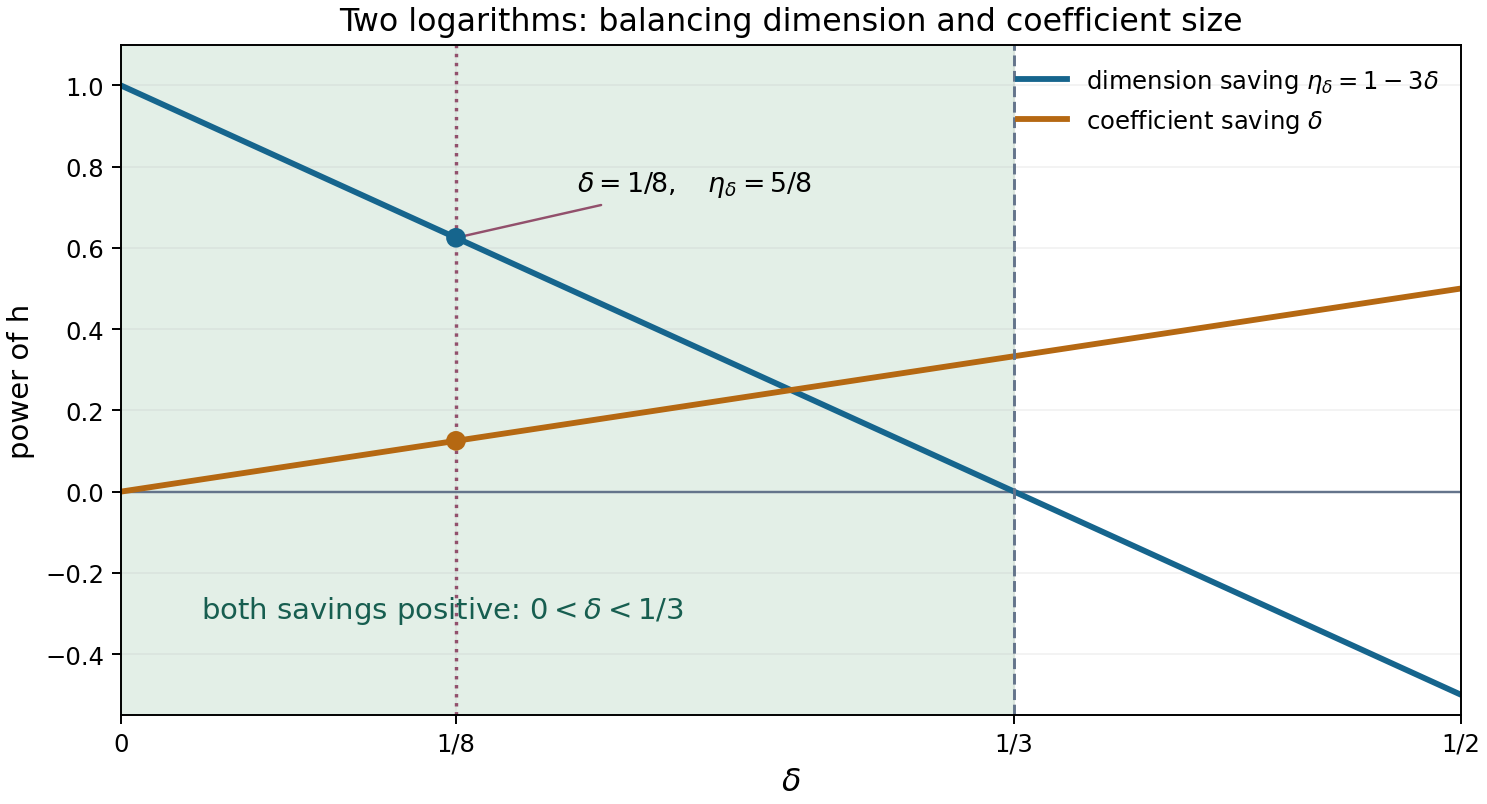
\includegraphics[keepaspectratio,alt={The two exponent savings for the two-logarithm auxiliary construction.}]{../figures/auxiliary-parameter-window.png}}
\par\smallskip
\begin{flushleft}\small
\emph{Figure.}
\end{flushleft}
\end{minipage}\par\medskip
 The sufficient parameter window (2.9) for \(n=2\). The
blue exponent \(\eta_\delta=1-3\delta\) controls the excess of unknowns:
\(N/M\ge h^{\eta_\delta}/(4D)\). The orange exponent \(\delta\) controls
the leading denominator contribution, whose ratio to \(h^3\) is
\(O(h^{-\delta})\). Both savings are positive for \(0<\delta<1/3\). At
the choice used in the proof, \(\delta=1/8\), they are \(1/8\) and
\(5/8\). The endpoints are excluded from this sufficient window; the
figure asserts no impossibility theorem at them. Original figure by
GPT-6.1 Sol (OpenAI), Codex, Ultra; CC0.
\href{../figure_sources/auxiliary_parameter_window.py}{Reproducible
figure source}.

For \(n=2,h=1000\), the chosen power \(h^{15/8}\) lies between
\(421696\) and \(421697\), so \(L=421696\). There are \(421697^3\)
unknowns and at most \(D\cdot1000\cdot1000001^2\) rational equations;
their ratio is about \(74.99/D\). This is a dimension example, not a
uniform assertion that \(h=1000\) meets the coefficient threshold for
every field and every algebraic relation.

\subsection{5. Growth and arithmetic separation at
integers}\label{growth-and-arithmetic-separation-at-integers}

For \(|m|\le h^2\), define the one-variable entire function

\[
f_m(z)=\partial^m\Phi(z,\ldots,z).
\]

\textbf{Proposition 2.3.} There are constants \(C_2,C_3>0\), independent
of \(h,m,z,l\), such that, for every sufficiently large \(h\),

\[
|f_m(z)|\le\exp\bigl(C_2(h^3+L|z|)\bigr)\quad(z\in\mathbb C), \tag{2.7}
\]

and, for every positive integer \(l\), either \(f_m(l)=0\) or

\[
|f_m(l)|\ge\exp\bigl(-C_3(h^3+Ll)\bigr). \tag{2.8}
\]

\textbf{Proof of the growth estimate.} The differentiated expression
(2.4) remains valid for complex \(z\) if its algebraic product is
interpreted as \(e^{z\sum_j\lambda_j\ell_j}\). Its exponential factor
has size at most \(e^{C L|z|}\). The powers of \(z\) are bounded by
\(\max(1,|z|)^L\le e^{L|z|}\). Formula (2.3), the factors
\(\gamma_r^{m_r}\), and the logarithmic prefactor have total size at
most \(e^{C h^2\log(L+1)}\). There are \((L+1)^{n+1}\) summands and
\(|p_\lambda|\le e^{h^3}\). Since \(h^2\log(L+1)=o(h^3)\), these bounds
imply (2.7).

\textbf{Proof of the arithmetic estimate.} Put
\(P_m=\prod_{r<n}\ell_r^{m_r}\ne0\). At a positive integer \(l\),

\[
A=q^{nLl+h^2}\frac{f_m(l)}{P_m}
\]

is an algebraic integer in \(K\), by exactly the denominator argument
used in Proposition 2.2. At every embedding
\(\sigma:K\hookrightarrow\mathbb C\), expand (2.4) after replacing the
algebraic data by their conjugates. There are finitely many fixed
conjugates, so the same estimates give

\[
|\sigma(A)|\le\exp\bigl(C_4(h^3+Ll)\bigr).
\]

Here \(L\log(l+1)\le L(l+1)\), and \(L\le h^2\), so the polynomial
factors are absorbed. If \(f_m(l)\ne0\), then \(A\ne0\), and its
rational integer norm has absolute value at least \(1\). Bound the other
\(D-1\) conjugates from above to obtain

\[
|A|\ge\exp\bigl(-(D-1)C_4(h^3+Ll)\bigr).
\]

Moreover \(\log|P_m|=\sum_{r<n}m_r\log|\ell_r|\ge-C_5h^2\), since the
logarithms are fixed and nonzero. Multiplying by \(|P_m|q^{-nLl-h^2}\)
gives (2.8). \(\square\)

The estimates have complementary directions. Complex analysis will make
\(f_m(l)\) extremely small at new integers. Arithmetic says a nonzero
value there has a definite minimum size. If the analytic estimate beats
that minimum, the new value is exactly zero.

\subsection{6. What changes when the constant term
vanishes}\label{what-changes-when-the-constant-term-vanishes}

If \(\beta_0=0\), no polynomial variable is needed. For \(n\ge2\),
define instead

\[
\Psi(z_1,\ldots,z_{n-1})
=\sum_{\lambda_1,\ldots,\lambda_n=0}^{L_0}
p_\lambda\prod_{r<n}e^{(\lambda_r+\lambda_n\beta_r)\ell_rz_r},
\qquad L_0=\left\lfloor h^{2-1/(4n)}\right\rfloor.
\]

The same diagonal algebraicity holds. There are \((L_0+1)^n\) unknowns
and at most \(D h(h^2+1)^{n-1}\) equations. The ratio grows at least as
a fixed positive multiple of \(h^{3/4}\). The coefficient bound and
growth/norm arguments therefore work with the same \(e^{h^3}\) scale.
This smaller construction explains why the inhomogeneous theorem
requires extra work.

\subsection{7. Exercises}\label{exercises}

\textbf{Exercise 1 (easy).} Assuming Theorem 2.1, prove the
Gelfond--Schneider theorem: if \(\alpha\ne0,1\) is algebraic and
\(\beta\) is algebraic irrational, every value of \(\alpha^\beta\) is
transcendental.

\textbf{Exercise 2 (medium).} Prove the coordinate bound in Section 4 by
multiplying integer matrices. Explain why it is valid even when the
algebraic generators are not a basis of the field.

\textbf{Exercise 3 (medium).} Verify the derivative formula (2.4) for
\(n=2\) and \(m=(2,1)\). Track every factor containing a logarithm.

\textbf{Exercise 4 (medium).} Prove that \(N/M\to\infty\) with the
parameter \(L\) used in Proposition 2.2. Give an explicit sufficient
inequality on \(h\) for \(N\ge2M\), in terms of \(D,n\). Explain why
this does not yet supply an explicit threshold for the coefficient
bound.

\textbf{Exercise 5 (hard).} Prove the auxiliary construction and both
estimates for the function \(\Psi\) in the constant-free case. Give the
denominator-clearing exponent and all equation and unknown counts.

\textbf{Exercise 6 (medium).} Suppose \(\alpha\) has degree \(d\) and
satisfies

\[
A_0\alpha^d+A_1\alpha^{d-1}+\cdots+A_d=0,
\qquad A_j\in\mathbb Z,\quad A_0\ne0,\quad |A_j|\le A,\quad A\ge1.
\]

Prove that, for every \(j\ge0\), the power \((A_0\alpha)^j\) is a linear
combination of \(1,\alpha,\ldots,\alpha^{d-1}\) with integer
coefficients of absolute value at most \((2A)^j\). This gives an
explicit one-generator counterpart of the matrix estimate in Section 2.

\subsection{8. Solutions}\label{solutions}

\textbf{Solution 1.} Choose a logarithm \(\ell\) of \(\alpha\); it is
nonzero because \(\alpha\ne1\). If \(\gamma=e^{\beta\ell}\) were
algebraic, then \(\beta\ell\) would be a logarithm of \(\gamma\). The
pair \(\ell,\beta\ell\) is rationally independent, since a nontrivial
rational relation would make \(\beta\) rational. Theorem 2.1 forbids the
algebraic relation \(\beta\ell-(\beta\ell)=0\), viewed as coefficients
\(\beta,-1\) on those two logarithms. Every branch is handled by its
chosen \(\ell\).

\textbf{Solution 2.} If \(v\) is an integral coordinate vector,
multiplication by a fixed algebraic integer is \(v\mapsto Mv\) for an
integer matrix \(M\). The row-sum norm gives
\(\|Mv\|_\infty\le c\|v\|_\infty\). Starting from the coordinates of
\(1\), induction bounds a product of \(t\) factors by \(c^{t+1}\). The
triangle inequality gives the sum bound. The generators are used as
multiplication operators on an integral basis of \(\mathcal O_K\); they
themselves need not be linearly independent.

\textbf{Solution 3.} Write the coefficient indices as \((a,b,c)\).
Differentiation in \(z_0\) twice contributes

\[
Q_{a,c,2}(z)=a(a-1)z^{a-2}
+2ac\beta_0z^{a-1}+c^2\beta_0^2z^a,
\]

with terms containing negative powers omitted when their falling
factorial vanishes. Differentiation in \(z_1\) once contributes
\((b+c\beta_1)\ell_1\). On the diagonal, the exponential is
\(e^{(b\ell_1+c\ell_2)z}\); at \(l\) this is
\(\alpha_1^{bl}\alpha_2^{cl}\). Thus
\(\partial_{z_0}^2\partial_{z_1}\Phi(l,l)\) equals \(\ell_1\) times the
sum of the algebraic terms
\(p_{a,b,c}Q_{a,c,2}(l)(b+c\beta_1)\alpha_1^{bl}\alpha_2^{cl}\). The
only remaining logarithmic factor is the common prefactor \(\ell_1\).

\textbf{Solution 4.} Section 4 gives \(N/M\ge h^{(3n-1)/(4n)}/(D2^n)\).
Therefore

\[
h\ge(2^{n+1}D)^{4n/(3n-1)}
\]

is sufficient for \(N\ge2M\). The entry bound \(U\) still involves
constants depending on the actual algebraic data, not only \(D,n\). A
coefficient threshold must also ensure \(\log(NU)\le h^3\); the
dimension inequality alone does not do that.

\textbf{Solution 5.} Divide the derivative
\(\partial^m\Psi(l,\ldots,l)\) by \(\prod_{r<n}\ell_r^{m_r}\). The
result is

\[
\sum_\lambda p_\lambda\prod_{j=1}^n\alpha_j^{\lambda_jl}
\prod_{r<n}(\lambda_r+\lambda_n\beta_r)^{m_r}.
\]

For \(l\le h\), \(|m|\le h^2\), multiplication by \(q^{nL_0h+h^2}\)
clears denominators. There are at most \(D h(h^2+1)^{n-1}\) integer
equations and \((L_0+1)^n\) unknowns. Their ratio is at least
\(h^{3/4}/(D2^{n-1})\). The entries obey
\(\log U\le C(L_0h+h^2\log(L_0+1)+h^2)\), whose ratio to \(h^3\) tends
to zero. Siegel's lemma therefore gives nonzero integer coefficients of
size at most \(e^{h^3}\). For complex \(z\), each differentiated summand
has exponential growth \(e^{CL_0|z|}\) and derivative factors
\(e^{Ch^2\log(L_0+1)}\), proving the growth estimate. At an arbitrary
positive integer \(l\), use \(q^{nL_0l+h^2}\) instead; its product with
the normalized value is an algebraic integer. Bounding all conjugates
and using its nonzero integer norm gives the arithmetic lower bound.
Restore the logarithmic prefactor, whose size is at least \(e^{-Ch^2}\).
Both estimates have the shapes (2.7)--(2.8).

\textbf{Solution 6.} Start at \(j=0\) with coefficient vector
\((1,0,\ldots,0)\). If \((A_0\alpha)^j=\sum_{k=0}^{d-1}c_k\alpha^k\),
multiplication by \(A_0\alpha\), followed by one use of the displayed
polynomial relation, gives new coefficients

\[
c'_0=-A_dc_{d-1},\qquad
c'_k=A_0c_{k-1}-A_{d-k}c_{d-1}\quad(1\le k<d).
\]

They are integers, and each has absolute value at most
\(2A\max_k|c_k|\). Induction proves the bound. For \(d=1\), only the
first formula is present and it gives the stronger factor \(A\).

\subsection{Prerequisites and
continuation}\label{prerequisites-and-continuation}

The integral-basis and norm facts are proved in the lessons cited in the
introduction. The stated integer-matrix form of Siegel's lemma is proved
in the written fifth lesson of \emph{Transcendental numbers}.
Proposition 2.2, both estimates in Proposition 2.3, the
arithmetic-coordinate calculation and all exercise solutions are proved
here. Theorem 2.1 is completed by extrapolation and coefficient recovery
in \href{../TR-BAKER-03.html}{\emph{Baker's theorem II: extrapolation
and the end of the proof}}; the Gelfond--Schneider deduction uses that
completed theorem.

\subsection{References}\label{references}

\begin{itemize}
\tightlist
\item
  {[}Waldschmidt 2003{]} Michel Waldschmidt, ``Linear Independence
  Measures for Logarithms of Algebraic Numbers,'' in \emph{Diophantine
  Approximation}, Lecture Notes in Mathematics 1819, Springer, 2003,
  249--344.
  \href{https://webusers.imj-prg.fr/~michel.waldschmidt/articles/pdf/SpringerLN1819-2003.pdf}{Author's
  full text}. Explains the normalized derivations, auxiliary
  construction and extrapolation, including nonhomogeneous forms.
\item
  {[}Waldschmidt 2000{]} Michel Waldschmidt, \emph{Diophantine
  Approximation on Linear Algebraic Groups}, Springer, 2000.
  \href{https://webusers.imj-prg.fr/~michel.waldschmidt/articles/pdf/dalag.pdf}{Author's
  full text}. Develops the height, Liouville and box-principle
  arguments.
\item
  {[}Sutherland 2021{]} Andrew V. Sutherland, \emph{Number Theory I},
  MIT OpenCourseWare, Fall 2021.
  \href{https://ocw.mit.edu/courses/18-785-number-theory-i-fall-2021/mit18_785f21_lec4.pdf}{Norm
  and trace} and
  \href{https://ocw.mit.edu/courses/18-785-number-theory-i-fall-2021/mit18_785f21_lec5.pdf}{integral
  lattices}. These notes are credited to Sutherland and MIT; their own
  licence applies.
\item
  {[}Waldschmidt 1992{]} Michel Waldschmidt, \emph{Linear Independence
  of Logarithms of Algebraic Numbers}, IMSc Report 116, 1992, revised
  text dated 2016.
  \href{https://webusers.imj-prg.fr/~michel.waldschmidt/articles/pdf/LIL.pdf}{Author's
  full text}. A complementary treatment using interpolation
  determinants.
\end{itemize}

\subsection{Editable source}\label{editable-source}

\href{TR-BAKER-02.md}{Markdown source}.

\end{document}
